\documentclass[12pt]{article}
\usepackage[utf8]{vietnam}
\usepackage{graphicx}
\begin{document}
\tableofcontents{}

\newpage
\section{Giới thiệu đề tài}
\subsection{Bối cảnh}
Trực quan dữ liệu, được hiểu là cách dùng hình ảnh để biểu diễn thông tin, ngày nay đã trở nên phổ dụng bởi những lợi ích nó mang lại.

Trực quan hóa khai thác hệ thống thị giác con người để cung cấp một cách trực quan, nhanh chóng, độc lập với ngôn ngữ để xem và hiển thị dữ liệu. Đây là công cụ đắc lực để phân tích và tìm hiểu thông tin. Cho đến nay, hệ thống thị giác con người là thứ đắt nhất, trực tiếp nhất, đem lại lượng thông tin lớn nhất lưu trong bộ nhớ con người. Lượng bộ nhớ tiêu tốn để xử lý thông tin thị giác vượt xa hơn so với những giác quan khác của con người. Một số nghiên cứu ước tính rằng hệ thống thị giác của con người có thể xử lý 9 megabit thông tin trên 1 giây, tương đương với gần 1 triệu kí tự trên 1 giây.

Mặc cho tiềm năng của nó, Trực quan dữ liệu vẫn chưa được đánh giá cao bởi sự thiếu hiểu biết về nó. Nhiều xu hướng ngày nay về Trực quan dữ liệu thực sự đã gây ra những tác dụng phụ mang tính tiêu cực, đó là sự nhầm lẫn thay vì thấu hiểu thực sự về Trực quan dữ liệu. 

Ngày nay trong lĩnh vực kinh doanh hiệu quả (Business Intelligence) không có gì có thể mang chúng ta lại gần hơn với những hứa hẹn về sự tương tác thông minh hơn là Trực quan dữ liệu. Nhưng điều này chỉ xảy ra khi chúng ta thực sự hiểu và dùng nó một cách đúng đắn. Để đạt được điều đó, chúng ta phải thực sự hành động và vứt bỏ những quan niệm chưa đúng về Trực quan dữ liệu.

Trực quan dữ liệu ngày càng đóng vai trò quan trọng trong mọi lĩnh vực đời sống. Như sử dụng trong nghiên cứu, trong những công việc liên quan tới xử lý dữ liệu, giao dịch bởi người dùng phổ thông, và dùng với tỷ lệ ngày càng tăng trong lực lượng lao động trí óc, đặc biệt đối với các nhà phân tích. Đó là những tin mang tính khởi sắc. Bên cạnh đó, vẫn còn những mặt hạn chế, trong giới doanh nghiệp, Trực quan dữ liệu vẫn còn bị bỏ ngỏ, hiểu nhầm, sử dụng chưa hiệu quả, và thường bị làm sai lệch đi bởi các nhà cung cấp, sản xuất và bán phần mềm trực quan. 

\subsection{Mục tiêu}
Trực quan dữ liệu đã trở thành một lĩnh vực nghiên cứu trong những năm gần đây. Nhiều trường đại học đã mở các Khoa chyên nghiên cứu về Trực quan và có một số chương trình ưu việt phục vụ nhu cầu nghiên cứu và chế tạo các nguyên mẫu của sinh viên. Cộng đồng nghiên cứu này bao gồm các cá nhân đến từ nhiều lĩnh vực không chỉ riêng Khoa học Máy tính, như tâm thần học và thậm chí các doanh nghiệp, nơi tạo môi trường lý tưởng để phát triển lý thuyết Trực quan một cách thực tế và mang tính cách mạng nhất.

Chúng ta đang bắt đầu nhận thấy các sản phẩm Trực quan dữ liệu đang thực sự tiện ích như thế nào. Khi một công ty có thể phân tích big data, họ sẽ được nhiều lợi ích. Trong một cuộc khảo sát [link bài báo], 63\% cho rằng họ tin tưởng việc hiểu biết và khai thác big data 1 cách hiệu quả có thể tạo ra lợi thế cạnh tranh cho tổ chức. Phân tích big data có thể giúp họ cải thiện việc ra quyết định, tạo ra 1 cái nhìn toàn diện về khách hàng của họ, tăng tính bảo mật và kiểm soát, phân tích hoạt động và gia tăng kho dữ liệu. Trực quan hóa có vai trò quan trọng trong việc sử dụng big data để có 1 cái nhìn đầy đủ về khách hàng của họ.

Bởi vì những lợi ích mà Trực quan hoá mang lại, dựa trên những công trình nghiên cứu liên quan, mục tiêu của đề tài là xây dựng một thư viện hỗ trợ người dùng có thể dễ dàng tiếp cận và xây dựng một ứng dụng để trực quan dữ liệu. Đồng thời, so sánh  đánh giá các phương pháp đã có để tìm ra mô hình thiết kế phù hợp.  

\section{Các công trình liên quan}
\subsection{Công cụ hỗ trợ trực quan dữ liệu phân tán Gapminder}
\subsubsection{Giới thiệu}
Gapminder được thành lập tại Stockholm bởi Ola Rosling, Anna Rosling Rönnlund và Hans Rosling vào ngày 25 tháng 2 năm 2005. 

Gapminder là một tổ chức phi lợi nhuận nhằm thúc đẩy sự phát triển bền vững toàn cầu, và là một thành tựu đánh dấu mục tiêu phát triển mang tầm thế kỷ của tổ chức Liên Hiệp Quốc (United Nations). Với mục tiêu đề ra nhằm gia tăng khả năng tìm hiểu, phân tích và đánh giá các thống kê , dữ liệu liên quan đến các vấn đề xã hội, tài chính và phát triển môi trường ở địa phương, quốc gia, và tầm thế giới.

Gapminder hoạt động dựa trên nền tảng được xác định trước, xây dựng các dịch vụ bởi ban quản trị, đôi khi hợp tác với các dự án  tại các trường đại học, các tổ chức quốc tế, cơ quan Nhà nước cũng như các tổ chức phi chính phủ.

\subsubsection{Mục tiêu}
\lq Fighting devastating ignorance with fact-based worldviews everyone can understand. [link] \rq 

Các hoạt động ban đầu là theo đuổi sự phát triển của ứng dụng Trendalyzer (tháng 3 năm 2006). Trendalyzer là một phần mềm biểu diễn chuỗi thời gian thống kê bằng cách chuyển đổi những con số khô khan, nhàm chán thành các đồ thị chuyển động thú vị, và đặc biệt là khả năng tương tác. Trendalyzer còn được biết đến dưới tên gọi Gapminder World, xây dựng trên nền tảng web biểu diễn dữ liệu thống kê theo dòng thời gian cho tất cả các quốc gia trên thế giới.

Gapminder World cung cấp các video, bài thuyết trình bằng Flash và các đồ thị dưới dạng PDF thể hiện xu hướng phát triển mang tính toàn cầu. 

Kể từ năm 2006 Gapminder cung cấp một lượng lớn các video thể hiện thực tế dưới góc nhìn toàn cầu. 

Từ năm 2008 Gapminder còn cung cấp các biểu đồ con (sub-graph) thể hiện xu hướng, sự khác biệt giữa các tiểu bang của Mỹ, các tỉnh thành của Trung Quốc, hay các đồ thị đặc biệt so sánh số liệu thống kê từ các thành phố ở Trung Quốc, Mỹ, Ấn Độ với các quốc gia khác trên thế giới. Từ Gapminder World, chỉ bằng một cú click chuột, các dữ liệu, thống kê liên quan nằm sau các đồ thị được thể hiện trên các biểu đồ con.

\begin{center}
    \begin{figure}[htp]
    \begin{center}
     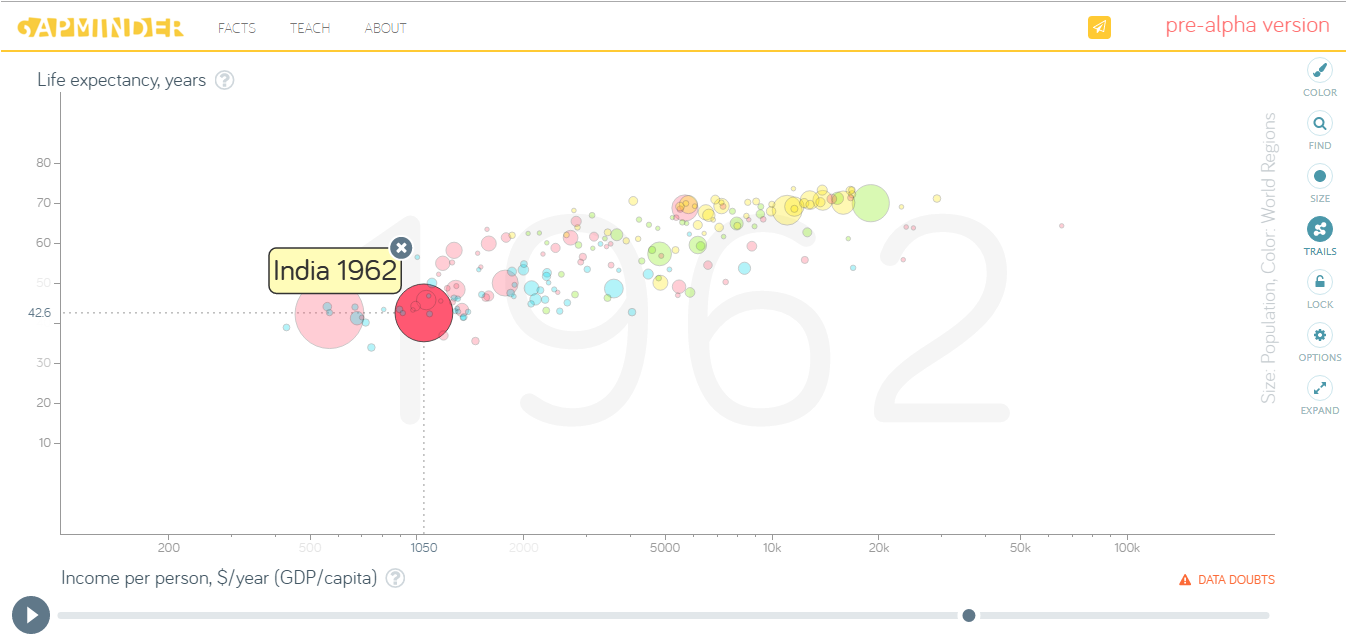
\includegraphics[scale=.4]{image/gapminder}
    \end{center}
    \caption{Đồ thị trực quan dữ liệu Gapminder World}
    \label{refhinh1}
    \end{figure}
\end{center}

\subsubsection{Phương pháp}
Gapminder sử dụng D3.js, một thư việc JavaScript phổ biến trong việc thao tác với các thành phần của một trang web (Document Object Model) dựa trên dữ liệu. 

D3 cho phép thể hiện dữ liệu thông qua HTML, SVG và CSS. D3 còn là một tiêu chuẩn web cung cấp hầu hết các khả năng mà một trình duyệt hiện đại mang lại, mà không cần phải tự viết lại hay dựa trên một nền tảng khuôn khổ. Kết hợp các thành phần trực quan mạnh mẽ và hướng tiếp cận dữ liệu để thao tác trên DOM.

\subsubsection{Đánh giá}
Với mục tiêu luôn luôn cập nhật các công cụ cũng như dữ liệu, nhằm đảm bảo tính xác thực, và đúng đắn của ứng dụng, Gapminder World đảm bảo nguồn dữ liệu chính xác nhất và cập nhật nhất.
Dữ liệu đề tài sẽ sử dụng từ Gapminder để đảm bảo nguồn thông tin luôn xác thực và thể hiện đúng đắn nhất các xu hướng phát triển toàn cầu.

Ngoài ra, cách sử dụng các biểu đồ con để hiển thị dữ liệu liên quan của một đối tượng được tương tác giúp người dùng dễ dàng nắm bắt được chính xác các thông tin muốn truyền đạt, tăng tính thân thiện cũng như trải nghiệm người dùng. Áp dụng tính hiệu quả trên, đề tài đề xuất sử dụng cách thể hiện trải nghiệm người dùng (UI/UX) kế thừa các đặc tính của Gapminder World. 

Về thư viện D3.js được sử dụng trong Gapminder World, đây là một thư viện mạnh mẽ tiếp cận dữ liệu dựa trên các thao tác với DOM. D3.js cho phép tái sử dụng các thành phần và trình nhúng (plugin) một cách đơn giản và hiệu quả. Đề tài đề xuất sử dụng D3.js làm thư viện chính để hiện thực thư viện tương tác giữa các đồ thị.

\subsection{Global Health Atlas - WHO}
\subsubsection{Giới thiệu}
Trong một môi trường điện tử, WHO’s Communicable Disease Global Atlas được dùng cho việc phân tích và so sánh dữ liệu chuẩn, thống kê các bệnh truyền nhiễm ở các quốc gia, vùng lãnh thổ, và toàn thế giới. Việc phân tích và biểu diễn dữ liệu ngày càng được hỗ trợ tốt hơn thông qua các thông tin về dân số, điều kiện kinh tế xã hội, và các yếu tố môi trường. Với việc làm đó, Atlas có thể biết được những yếu tố gây ra bệnh truyền nhiễm.

\begin{center}
    \begin{figure}[htp]
    \begin{center}
     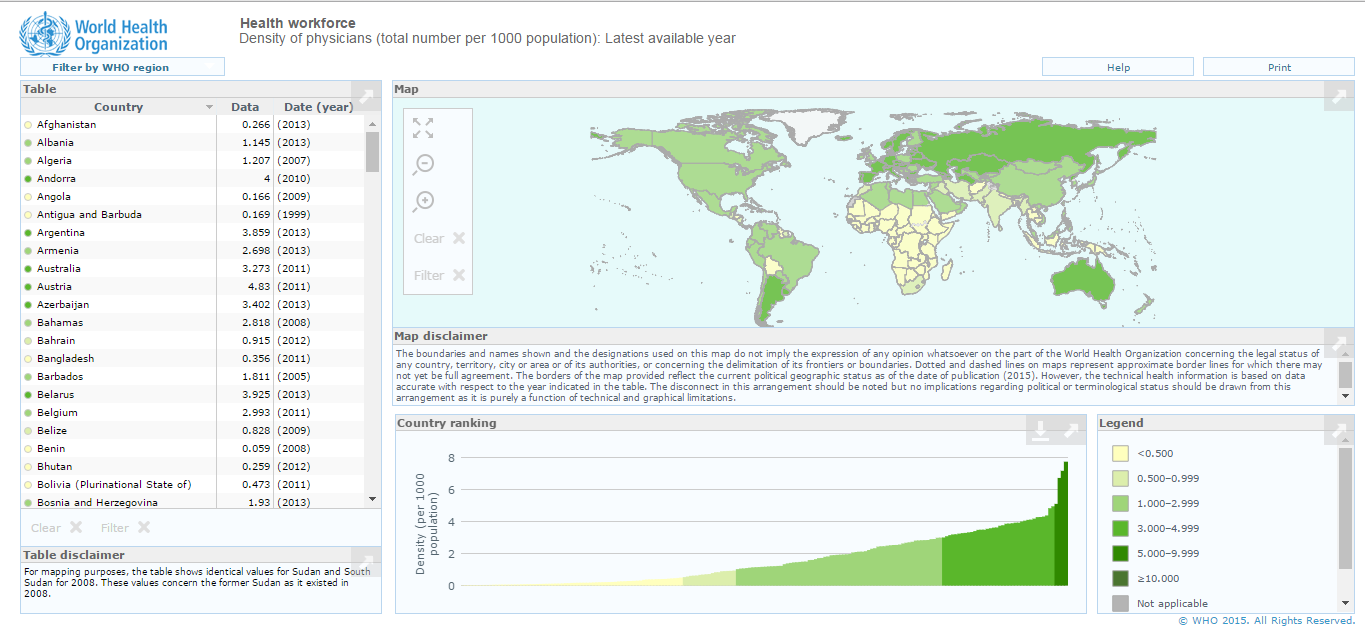
\includegraphics[scale=.4]{image/globalatlas}
    \end{center}
    \caption{Biểu đồ tương tác về mật độ bác sĩ của WHO}
    \label{refhinh2}
    \end{figure}
\end{center}

\subsubsection{Mục tiêu}
Ban đầu, với mục đích cung cấp những dữ liệu, báo cáo về các bệnh truyền nhiễm chính (sốt rét, HIV/AIDS,..), thì ngày nay Global Atlas của WHO cũng dùng để phân tích, biểu diễn, so sánh dữ liệu từ những vấn đề liên quan đến y tế khác như: mật độ bác sĩ, số lượng người chết do tai nạn giao thông, tuổi thọ trung bình,… 

\subsubsection{Phương pháp}
Trực quan dữ liệu thành nhiều dạng biểu đồ khác nhau, các biểu đồ có thể tương tác với nhau giúp cho việc nhìn nhận, phân tích, đánh giá thông tin một cách chính xác, đầy đủ.

Ứng dụng bao gồm các thành phần:

\indent \indent \textbullet \ Bảng dữ liệu: được lấy từ database của WHO

\indent \indent \textbullet \ Map: dùng thư viện Google Maps, kết hợp với bảng dữ liệu để tạo ra biểu đồ

\indent \indent \textbullet \ Biểu đồ cột: dựa vào bảng dữ liệu để tạo ra biểu đồ

\indent \indent \textbullet \ Chú thích: phân vùng dữ liệu

Tính năng: ứng dụng hỗ trợ tương tác giữa các biểu đồ, bảng dữ liệu:

\indent \indent \textbullet \ Khi click vào 1 hàng trong bảng dữ liệu, bên map sẽ phóng to đến vùng tương ứng, bên biểu đồ cột sẽ nổi bật cột tương ứng. Các tương tác sẽ được thể hiện tương tự khi click vào các biểu đồ.
\begin{center}
    \begin{figure}[htp]
    \begin{center}
     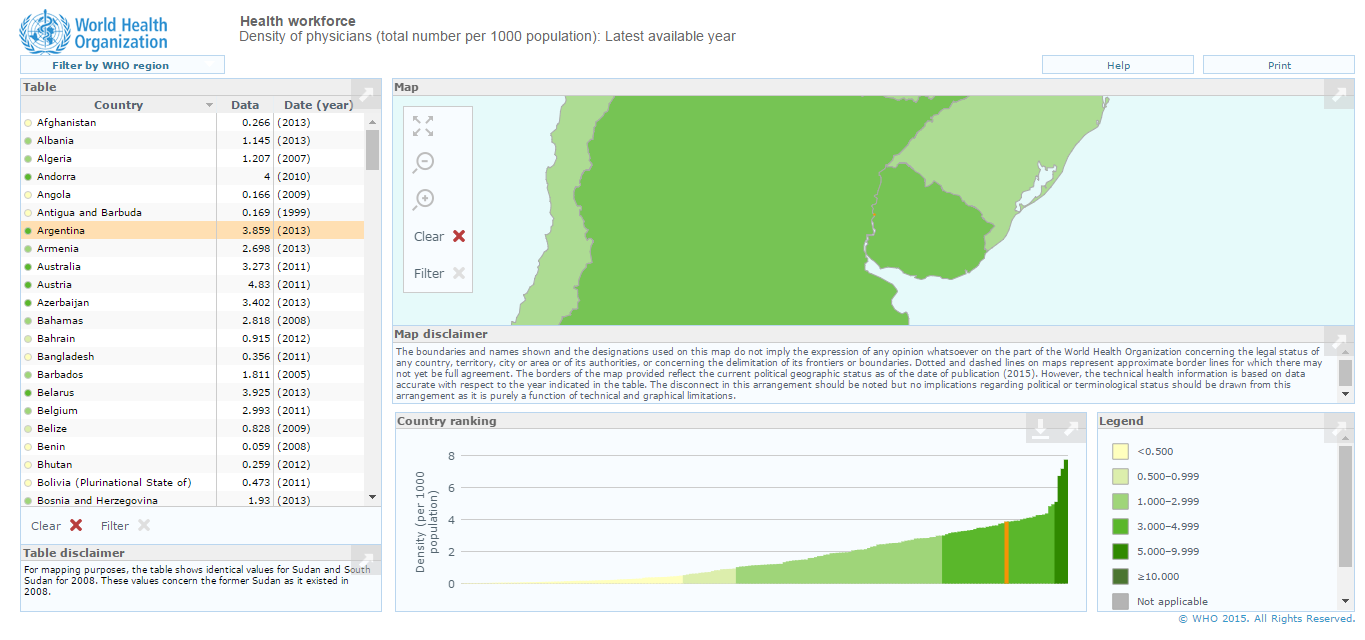
\includegraphics[scale=.4]{image/clickatlas}
    \end{center}
    \caption{Tương tác khi click vào một hàng trong bảng dữ liệu}
    \label{refhinh3}
    \end{figure}
\end{center}
\indent \indent \textbullet \ Khi hover lên 1 hàng trong bảng dữ liệu, bên các biểu đồ cũng sẽ được làm nổi bật vùng tương ứng như khi click, nhưng với 1 màu sắc khác (bên map sẽ không phóng to đến vùng tương ứng).
\begin{center}
    \begin{figure}[htp]
    \begin{center}
     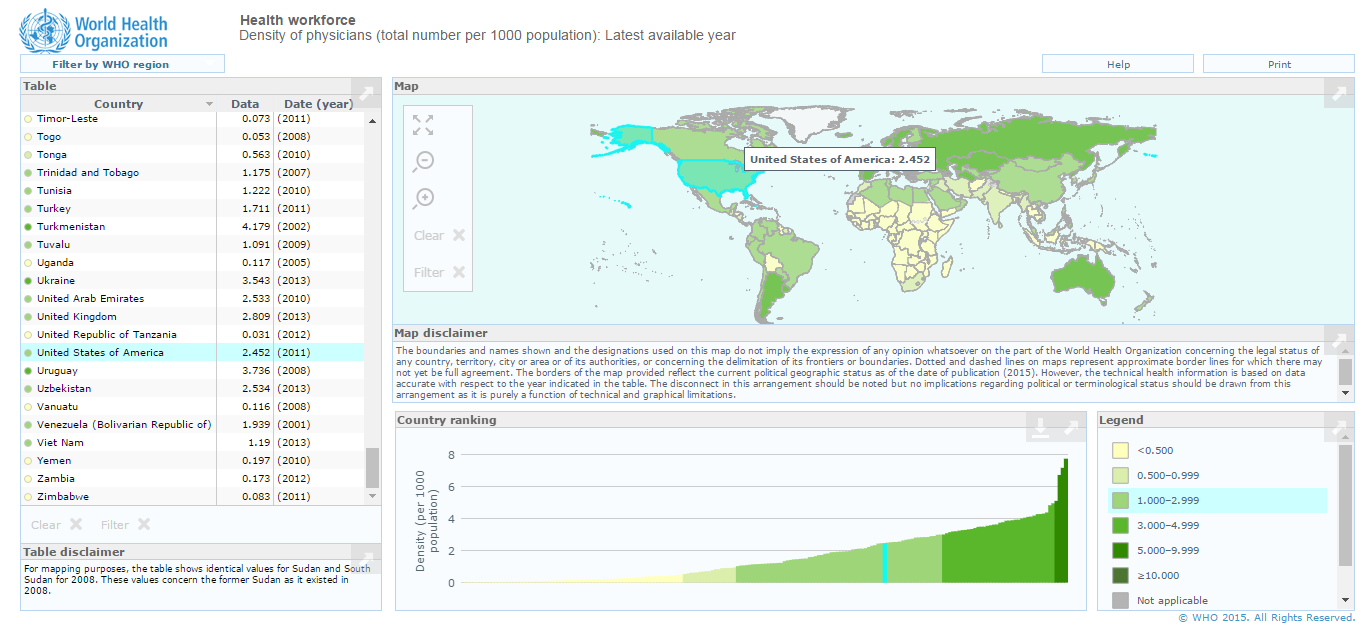
\includegraphics[scale=.4]{image/hoveratlas}
    \end{center}
    \caption{Tương tác khi hover lên Map}
    \label{refhinh4}
    \end{figure}
\end{center}
\subsubsection{Đánh giá}
Dữ liệu được WHO thu thập trên toàn thế giới, cập nhật theo thời gian, đảm bảo tính chính xác của ứng dụng.

Bên cạnh đó, việc trực quan thành nhiều loại biểu đồ, thể hiện được nhiều cái nhìn khác nhau của dữ liệu giúp đánh giá vấn đề 1 cách đúng đắn, đầy đủ.

Một tính năng khác đó là việc tương tác giữa các giữa các đồ thị giúp người dùng có nhiều cái nhìn từ nguồn dữ liệu, hiểu được thông tin rút trích từ các đồ thị, tăng tính thân thiện, trải nghiệm của người dùng.

Do đó, đề tài đề xuất sử dụng nhiều đồ thị để biểu diễn cho nguồn dữ liệu đầu vào, và sự tương tác giữa các đồ thị.


\end{document}